
In this section, we answer the first two research questions on the extent to which the selected crashes and their frames were reproduced and the impact of the project and the exception type on the performance of \evocrash.
%
We detail the results by analyzing the outcome of \evocrash  in a majority of 10 executions for each frame of each stack trace. We classify the outcome of each execution in one of the five following categories:
\begin{itemize}
\item[] \textbf{reproduced:} when \evocrash generated a test that successfully reproduced the stack trace at the given frame level; 
\item[]\textbf{ex. thrown:} when \evocrash generated a test that cannot fully reproduce the stack trace, but covers the target line and throws the desired exception. The frames of the exception thrown, however, do not contain all the original frames;
\item[]\textbf{line reached:} when  \evocrash generated a test that covers the target line, but does not throw the desired exception;
\item[]\textbf{line not reached:} when none of the tests produced by \evocrash could cover the target line within the available time budget;
and \item[]\textbf{aborted:} when \evocrash could not generate an initial population to start the search process.
\end{itemize}
%
Each outcome denotes a particular state of the search process. For the \emph{reproduced} frames, \evocrash could generate a crash-reproducing test within the given time budget (here, 62,328 fitness evaluations). For the frames that could not be reproduced, either \evocrash exhausted the time budget (for \emph{ex. thrown}, \emph{line reached}, and \emph{line not reached} outcomes) or could not perform the guided initialization (i.e., generate at least one test case with the target method) and did not start the search process (\emph{aborted} outcomes). 
For instance, if the class in the target frame is abstract, \evocrash may fail to find an adequate implementation of the abstract class to instantiate an object of this class during the guided initialization.

\subsection{Crash Reproduction Outcomes (RQ1)}

For \textbf{RQ$_1$},  we first look at the reproduced and non-reproduced crashes to answer \textbf{RQ$_{1.1}$}. 
If \evocrash was successful in reproducing any frame of a stack trace in a majority of 10 executions, we count the crash as a \textbf{reproduced crash}. Otherwise, we count the crash as \textbf{not reproduced}.
%
To answer \textbf{RQ$_{1.2}$}, we detail the results by analyzing the outcome of \evocrash  in a majority of 10 executions for each frame of each stack trace. 

\begin{figure}[t]
	\centering
%	\includegraphics[width=0.90\textwidth]{rq1_compact.pdf}
	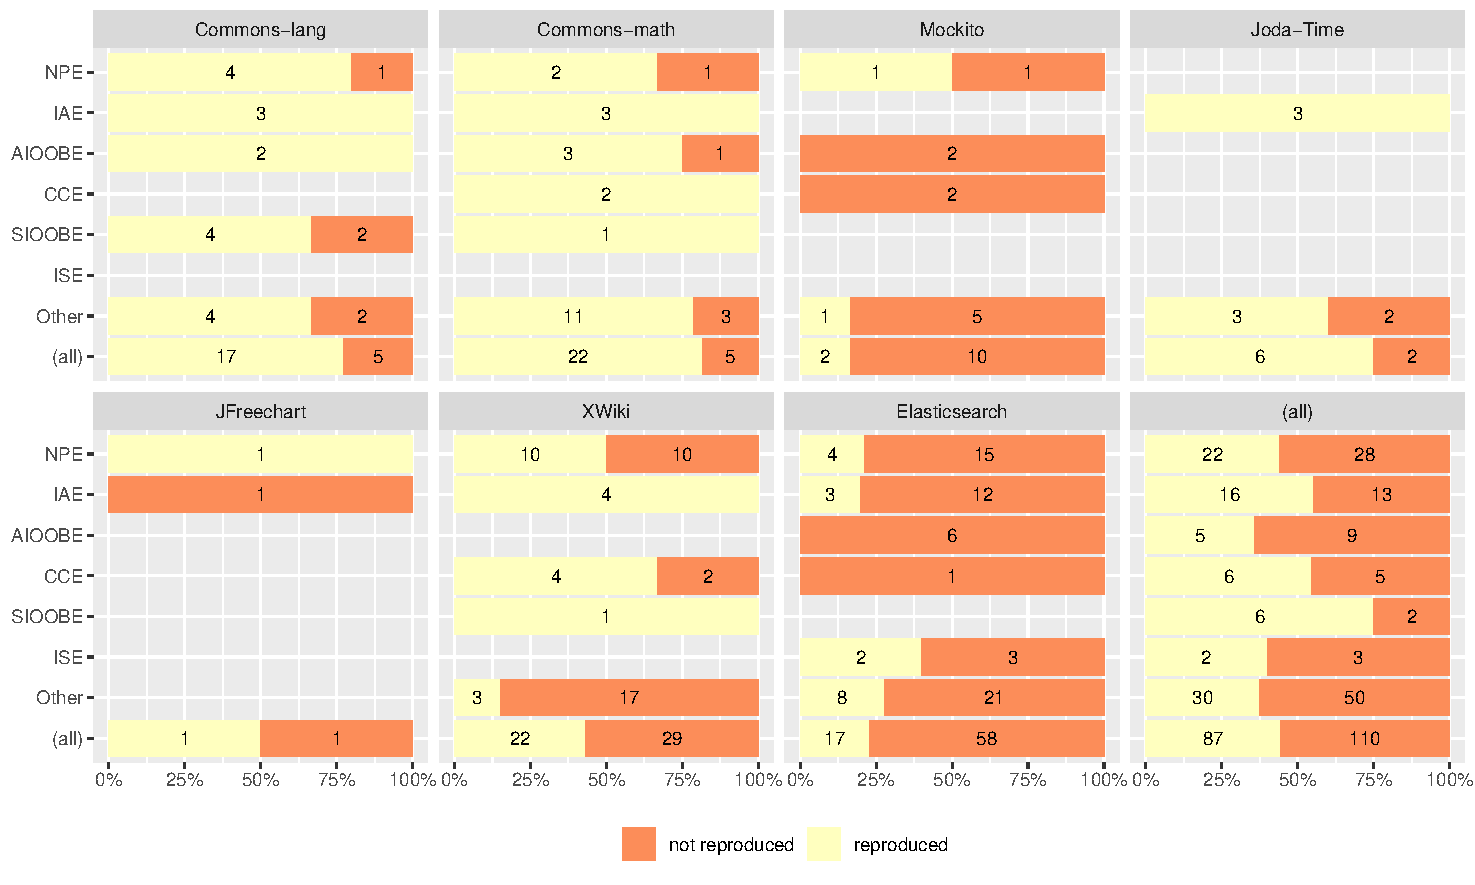
\includegraphics[width=\textwidth]{papers/jcrashpack/rq1_crashes.pdf}
	\caption{Reproduction outcome for the different crashes}
	\label{fig:rq1crashes}
\end{figure}

Figure \ref{fig:rq1crashes} shows the number of reproduced and not reproduced crashes for each project (and all the projects) and type of exception.
\evocrash is successful in reproducing the majority of crashes (more than 75\%) from \textit{Commons-lang}, \textit{Commons-math}, and \textit{Joda-Time}. 
For the other projects, \evocrash reproduced 50\% or less of the crashes, with only 2 out of 12 crashes reproduced for \textit{Mockito}.
%
Crashes with an \textit{IllegalArgumentException} are the most frequently reproduced crashed: 16 out of 29 (55\%).

\begin{figure*}[t]
	\centering
	\subfloat[In each type of exception]{
	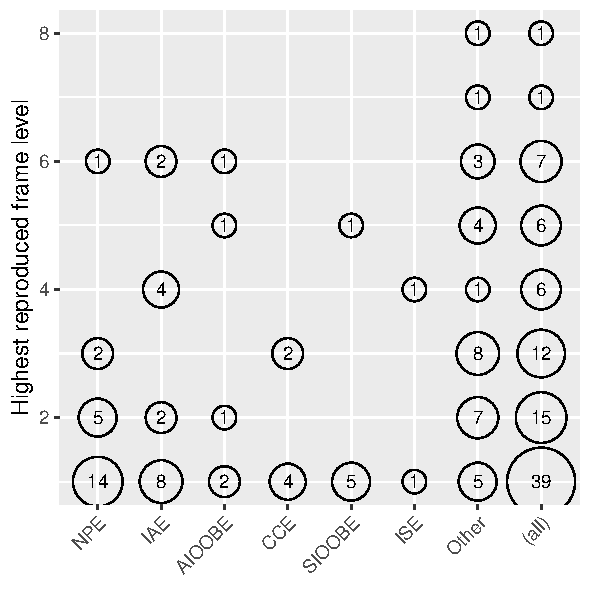
\includegraphics[width=0.48\textwidth]{papers/jcrashpack/rq1_framelvlex.pdf}
	\label{fig:rq1_framelvlex}
	}
	%
	\subfloat[In each type of application]{
	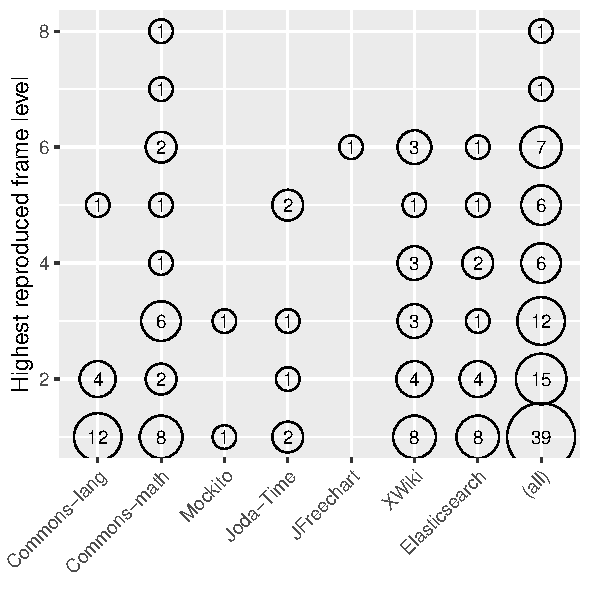
\includegraphics[width=0.48\textwidth]{papers/jcrashpack/rq1_framelvlapp.pdf}
	\label{fig:rq1_framelvlapp}
	}
	\caption{Highest reproduced frame levels}
	\label{fig:highestframe}
\end{figure*}

Before detailing the results of each frame of each crash, we first look at the frame levels that could be reproduced. Figure \ref{fig:highestframe} presents for the 87 stack traces that could be reproduced, the distribution of the highest frame level that could be reproduced for the different crashes for each type of exception (in Figure \ref{fig:rq1_framelvlex}) and each application (in Figure \ref{fig:rq1_framelvlapp}).
As we can see, \evocrash replicates lower frame levels more often than higher levels. 
For instance, for 39 out of  the 87 reproduced stack traces, \evocrash could not reproduce frames beyond level 1 and could reproduce frames up to level 5 for only 9 crashes. 

Figure \ref{fig:rq1_framelvlex} indicates that \evocrash can replicate only the first frame in 14 out of 22 NPE crashes, while there is only one NPE crash for which \evocrash could reproduce a frame above level 3. 
In contrast, it is more frequent for \evocrash to reproduce higher frame levels of IAE stack traces: the highest reproduced frames in 6 out of 16 IAE crashes are higher than 3.
%
Those results suggest that, when trying to reproduce a crash, propagating an illegal argument value trough a chain of method calls (i.e., the frames of the stack trace) is easier than propagating a \texttt{null} value. 
%
According to Figure \ref{fig:rq1_framelvlapp}, \evocrash can reproduce frames higher than 6 only for \textit{Commons-math} crashes. The highest reproduced frames in most of the reproduced crashes in this project are higher than level 2 (12 out of 22). 
In contrast, for \textit{Elasticsearch} the highest reproduced frame is 1 in most of the crashes.

Both the number of crashes reproduced and the highest level at which crashes could be reproduced confirm the relevance of our choice to consider crashes from XWiki and Elasticsearch, for which the average number of frames (resp. 27.5 and 17.7) is higher than for Defects4J projects (at most 6.0 for JFreeChart), as they represent an opportunity to evaluate and understand current limitations. 

\subsubsection{Frames reproduction outcomes} 

\begin{figure}[t]
	\centering
%	\includegraphics[width=0.90\textwidth]{rq1_compact.pdf}
	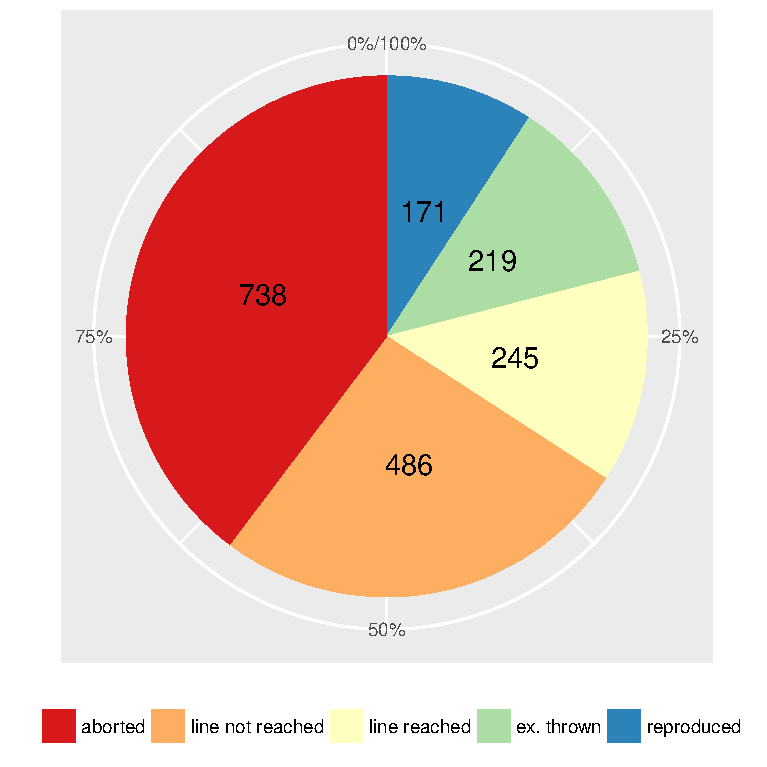
\includegraphics[width=8cm]{papers/jcrashpack/rq1_summary.pdf}
	\caption{An overview of the reproduction outcome}
	\label{fig:rq1summary}
\end{figure}

\begin{figure}[t]
	\centering
%	\includegraphics[width=0.90\textwidth]{rq1_compact.pdf}
	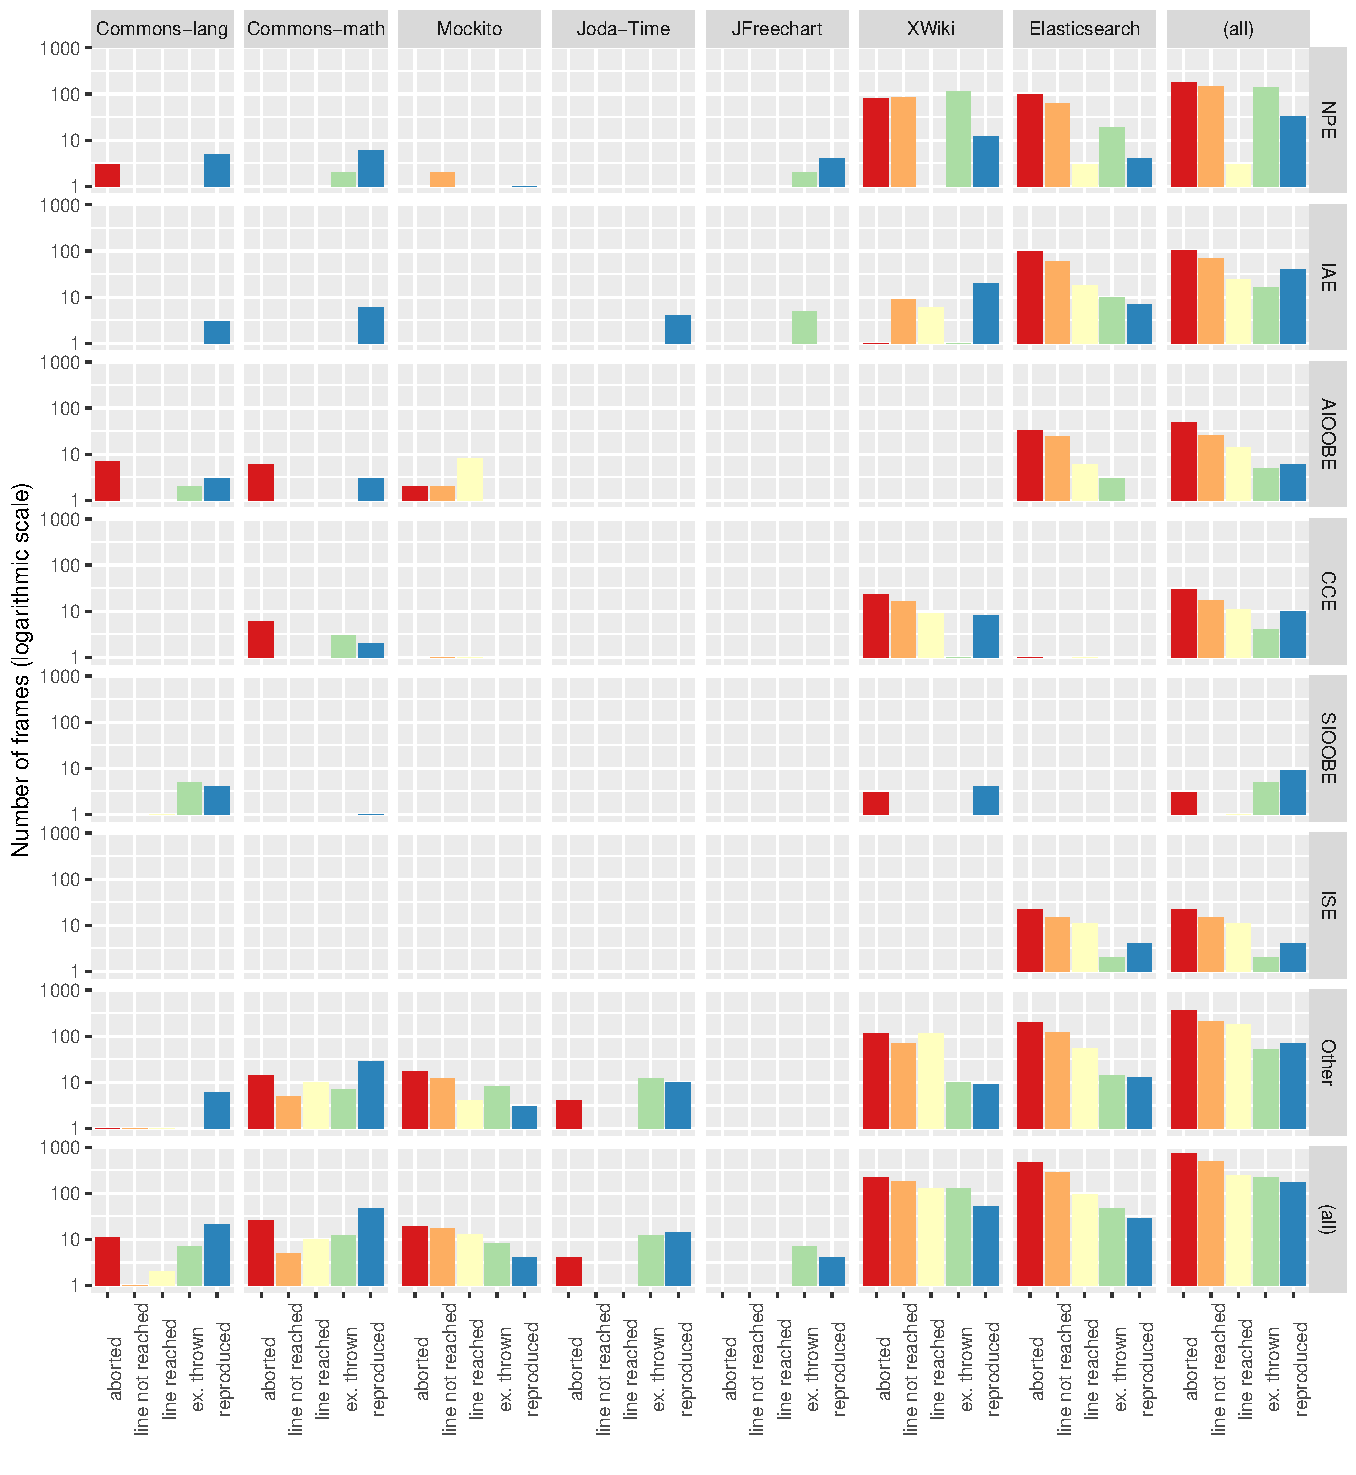
\includegraphics[width=\textwidth]{papers/jcrashpack/rq1_all.pdf}
	\caption{Detailed reproduction outcome for the different frames.}
	\label{figure:outcomecomp}
\end{figure}

To answer \textbf{RQ$_{1.2}$}, we analyze the results for each frame individually.
%
Figure~\ref{fig:rq1summary} presents a summary of the results with the number of frames for the different outcomes. Figure \ref{figure:outcomecomp} details the same results by application and exception. 

Overall, we see in Figure \ref{fig:rq1summary} that \evocrash reproduced 171 frames (out of 1,859), from 87 different crashes (out of 200) in the majority of the ten rounds. If we consider the frames for which \evocrash generated a crash-reproducing test at least once in the ten rounds, the number of reproduced frames increases to 201 (from 96 different crashes).
%
In total, \evocrash exhausted the time budget for 950 frames: 219 with a test case able to throw the target exception, 245 with a test case able to reach the target line, and 486 without a test case able to reach the line. 
\evocrash aborted the search for 738 frames, 455 of which were from Elasticsearch, the application for which \evocrash had the most difficulties to reproduce a stack trace. 

Figure~\ref{figure:outcomecomp} details the results by applications (columns) and exceptions (lines). The last line (resp. column), denoted \textit{(all)}, provides the global results for the applications (resp. exceptions). In the remainder of this section, we discuss the results for the different applications and exceptions. 

\subsubsection{Defects4J applications}

For the Defects4J applications, presented in the first five columns in Figure~\ref{figure:outcomecomp}, in total, 90 (out of 244) of the frames from 48 (out of 71) different crashes were \emph{reproduced}. 
For 94 frames, \evocrash exhausted the time budget (46 \emph{ex. thrown}, 25 \emph{line reached}, and 23 \emph{line not reached}) and \emph{aborted} for 60 frames from the Defects4J projects. 

In particular, only 4 frames out of 61 frames for Mockito were successfully reproduced.
For instance, \evocrash could not reproduce \texttt{MOCKITO-4b}, which has only one frame.
From our evaluation, we observe that one very common problem when trying to reproduce a \textit{ClassCastException} is to find which class should be used to trigger the exception.
%
\begin{lstlisting}[language=Java]
public void noMoreInteractionsWantedInOrder(Invocation undesired){
  throw new VerificationInOrderFailure(join( ...,
		"..." + undesired.getMock() + "':", ...));
}
\end{lstlisting}
%
The exception happens when the \texttt{undesired.getMock()} call returns an object that cannot be cast to \texttt{String}.
During the search, \evocrash mocks the \texttt{undesired} object and assigns some random value to return when the \texttt{getMock} method is called. 
\evocrash generates a test able to cover the target line, but failing to trigger an exception. 
Since the signature of this method is \texttt{Object getMock()}, \evocrash assigns only random \texttt{Object} values to return, where, from the original stack trace, a \texttt{Boolean} value is required to trigger the exception.

\subsubsection{XWiki and Elasticsearch}

XWiki is one of the industrial open source cases in the evaluation, for which 53 (out of 706) frames were successfully \emph{reproduced}, 430 could not be reproduced with the given time budget (125 \emph{ex. thrown}, 127 \emph{line reached}, and 178 \emph{line not reached}), and 223  \emph{aborted} during the generation of the initial population.
%
\evocrash \emph{reproduced} only 28 (out of 909) frames from Elasticsearch, for which, the majority of frames (455) \emph{aborted}  during the generation of the initial population. However, \evocrash was able to start the search for 426 frames (48 \emph{ex. thrown}, 93 \emph{line reached}, and 285 \emph{line not reached}).

\paragraph{Variability of the reproductions.}

We also observed that XWiki and Elasticsearch have the highest variability in their outcomes. 
For XWiki (resp. Elasticsearch), 4 (resp. 3) frames that could be reproduced in a majority of time could however not be reproduced 10 out of 10 times, compared to 2 frames for Commons-lang and Commons-math. 
This could indicate a lack of guidance in the current fitness function of \evocrash. 
For instance, for the Elasticsearch crash ES-26833, \evocrash could only reproduce the third frame 4 times out of 10 and was therefore not considered as reproduced. 
After a manual inspection, we observed that \evocrash gets stuck after reaching the target line and throwing the expected exception. 
From the intermediate test cases generated during the search, we see that the exception is not thrown by the target line, but a few lines after. 
Since the fitness value improved, \evocrash got stuck into a local optima, hence the lower frequency of reproduction  for that frame.\footnote{A detailed analysis is available at \url{https://github.com/STAMP-project/EvoCrash-JCrashPack-application/blob/master/results/manual-analysis/Elasticsearch/ES-26833.md}}
Out future work includes improvement of the guidance in the fitness function and a full investigation of the fitness landscape to decrease the variability of \evocrash outcomes. 


\paragraph{Importance of large industrial applications.}

Compared to Defects4J and XWiki applications, the crash reproduction rate drops from 36.9\% for Defects4J, to 7.5\% for XWiki, and only 3\% for Elasticsearch. Those results emphasize the importance of large industrial applications for the assessment of search-based crash reproduction and enforce the need of context-driven software engineering research to identify relevant challenges \cite{Briand2017a}. 

Additionally to the larger variability of reproduction rate, we observe that frequent use of \textit{Java generics} and \textit{static initialization}, and most commonly, automatically generating suitable input data that resembles \texttt{http} requests are among the major reasons for the encountered challenges for reproducing Elasticsearch crashes.
In Section~\ref{sec:jcrashpack:challenges} we will describe \textbf{14} categories of challenges that we identified as the underlying causes for the presented execution outcomes.

\subsubsection{Exceptions}

The lines in Figure~\ref{figure:outcomecomp} presents the outcomes for the different exceptions. In particular, NPE, IAE, AIOOBE, and CCE are the most represented exceptions in \crashpack. For those exceptions, \evocrash could reproduce, respectively, 32 (out of 499), 40 (out of 250), 6 (out of 99), and 10 (out of 72) frames. Looking at the reproduction frequency, IAE is the most frequently reproduced exception (16\%), followed by CCE (13.8\%), NPE (6.4\%), and AIOOBE (6\%). 

This contrast with the number of frames for which \evocrash aborted the search, where NPE has the lowest frequency (181 frames, 36.2\%), followed by IAE (101 frames, 40.4\%), CCE (30 frames, 41.6\%), and AIOOBE (48 frames, 48.4\%). Interestingly, those numbers show that \evocrash is able to complete the guided initialization for NPEs more often than for other exceptions. 

Figure~\ref{figure:outcomecomp} also shows that the number of test cases that reach the line is low for NPEs, meaning that whenever \evocrash generates at test able to cover the line (\emph{line reached}), the evolution process will be able to progress and generate another test that throws an exception (\emph{ex. thrown}).


\paragraph{\textbf{Summary (RQ$_1$)} To what extent can \evocrash reproduce crashes from \crashpack, and how far it can proceed in the stack traces?}
%
Overall, \evocrash reproduced 171 frames (out of 1,859 - 9\%), from 87 different crashes (out of 200 - 43.5\%) in a majority out of 10 executions. Those numbers climb to 201 frames (10.8\%) from 96 crashes (48\%) if we consider at least one reproduction in one of the 10 executions.
%
In most of the reproduced crashes, \evocrash can only reproduce the first two frames. It indicates that since \evocrash needs higher accuracy in setting the state of the software under test for reproducing higher frames, increasing the length of the stack trace reduces the chance of this tool for crash reproduction. 
%
When looking at larger industrial applications, the crash reproduction rates drop from 36.9\% for Defects4J to 7.5\% for XWiki and 3\% for Elasticsearch.
%
The most frequently reproduced exceptions are IllegalArgumentExceptions. The exceptions for which \evocrash is the most frequently able to complete the guided initialization are NullPointerExceptions.


\subsection{Impact of Exception Type and Project on Performance (RQ2)}

To identify the distribution of fitness evaluations per exception type and project, we filtered the \emph{reproduced} frames out of the 10 rounds of execution.
Tables~\ref{tab:appstats} and~\ref{tab:typestats} present the statistics for these executions, grouped by application and exception types, respectively.

\begin{table*}[t]
\caption{Statistics for the average number of fitness evaluations for the \textit{reproduced} frames (\textbf{fr}) belonging to different stack traces (\textbf{st}), grouped by \textbf{applications}, out of 10 rounds of execution.
The confidence Interval (\textbf{CI}) is calculated for the median bootstrapping with \textit{100,000} runs, at a 95\% confidence level.}
\label{tab:appstats}
\begin{scriptsize}
\begin{tabularx}{0.945\textwidth}{ l r r r r r r r r } 
\hline 
\textbf{Applications} & \textbf{st} & \textbf{fr}& \textbf{Min} & \textbf{Lower Quart.} & \textbf{Median CI} & \textbf{Med.} & \textbf{Upper Quart.} & \textbf{Max} \\ 
\hline 
\textbf{ Com.-lang } & 19  & 213  & 1  & 2.0  & [ 5.0 ,22.0] & 15.0  & 237.0  & 52,240  \\ 
\textbf{ Com.-math } & 24  & 471  & 1  & 13.0  & [ 124.0 ,211.0] & 178.0  & 1,046.5  & 58,731  \\ 
\textbf{ Mockito } & 2  & 40  & 1  & 1.0  & [ 1.0 ,1.0] & 1.0  & 5.2  & 138  \\ 
\textbf{ Joda-Time } & 6  & 138  & 1  & 15.5  & [ 79.1 ,369.0] & 253.5  & 1,290.2  & 40,189  \\ 
\textbf{ JFreechart } & 1  & 41  & 1  & 10.0  & [ -292.0 ,350.0] & 221.0  & 1,188.0  & 20,970  \\ 
\textbf{ XWiki } & 25  & 531  & 1  & 2.5  & [ 14.0 ,30.0] & 23.0  & 209.0  & 34,089  \\ 
\textbf{ Elasticsearch } & 19  & 287  & 1  & 4.0  & [ 5.0 ,32.0] & 23.0  & 125.0  & 17,461  \\ 
\hline 
\textbf{Total} & 96  & 1721  & 1  & 4.0  & [ 34.0 ,59.0] & 48.0  & 534.0  & 58,731  \\ 
\hline 
\end{tabularx} 

\end{scriptsize}
\end{table*}

\begin{table}[t]
\caption{Statistics for the average number of fitness evaluations for the \textit{reproduced} frames (\textbf{fr}) belonging to different stack traces (\textbf{st}), grouped by \textbf{exceptions}, out of 10 rounds of execution.
Confidence Interval (\textbf{CI}) is calculated for median with bootstrapping with \textit{100,000} runs, at 95\% confidence level.}
\label{tab:typestats}
\begin{scriptsize}
\begin{tabularx}{0.94\textwidth}{ l r r r r r r r r} 
\hline 
\textbf{Applications} & \textbf{st} & \textbf{fr}& \textbf{Min} & \textbf{Lower Quart.} & \textbf{Median CI} & \textbf{Med.} & \textbf{Upper Quart.} & \textbf{Max} \\ 
\hline 
\textbf{ NPE } & 26  & 330  & 1  & 6.0  & [ 9.0 ,63.0] & 44.5  & 220.0  & 34,089  \\ 
\textbf{ IAE } & 16  & 399  & 1  & 2.0  & [ 7.0 ,12.0] & 10.0  & 49.0  & 38,907  \\ 
\textbf{ AIOOBE } & 5  & 58  & 1  & 15.5  & [ 252.0 ,1,104.5] & 675.0  & 1,671.2  & 53,644  \\ 
\textbf{ CCE } & 6  & 103  & 1  & 6.5  & [ 74.0 ,210.0] & 120.0  & 560.0  & 10,197  \\ 
\textbf{ SIOOBE } & 8  & 95  & 1  & 12.5  & [ 122.0 ,945.0] & 505.0  & 2,326.0  & 52,240  \\ 
\textbf{ ISE } & 2  & 42  & 1  & 1.0  & [ 1.0 ,3.0] & 2.0  & 105.8  & 1,138  \\ 
\textbf{ Other } & 33  & 694  & 1  & 7.0  & [ 99.0 ,139.0] & 125.5  & 825.0  & 58,731  \\ 
\hline 
\textbf{Total} & 96  & 1721  & 1  & 4.0  & [ 34.0 ,59.0] & 48.0  & 534.0  & 58,731  \\ 
\hline 
\end{tabularx} 

\end{scriptsize}
\end{table}

We filtered out the frames that were not reproduced to analyze the impact of project and exception types on the average number of fitness evaluations and, following recommendations by Arcuri and Briand~\cite{Arcuri2014}, we replaced the test of statistical difference by a confidence interval.
For both groups, we calculated confidence intervals with a  $95\%$ confidence level for medians with bootstrapping with $100,000$ runs.\footnote{We used the \textit{boot} function from the \textit{boot} library in R to compute the \textit{basic} intervals with bootstrapping. See \url{https://github.com/STAMP-project/EvoCrash-JCrashPack-application/tree/master/results} to reproduce the statistical analysis.}

As Table~\ref{tab:appstats} shows, for four projects (Commons-lang, Mockito, XWiki, and Elasticsearch) the median number of fitness evaluations is low.
On the contrary, the cost of crash reproductions for Commons-math, Joda-Time, and JFreechart are  higher in comparison to the rest of projects.
By comparing those results with the projects sizes reported in Table \ref{tab:benchmark:complexity}, where the largest projects are XWiki (with $\overline{NCSS}=177.84k$) and Elasticsearch (with $\overline{NCSS}=124.36k$), we observe that the effort required to reproduce a crash cannot be solely predicted by the project size. 
This is consistent with the intuition that the difficulty of reproducing a crash only depends on the methods involved in the stack trace.

Similarly, according to Figure \ref{fig:ccnperapp}, the average CCN for Mockito, XWiki, and Elasticsearch is lower compared to other projects. 
Table~\ref{tab:appstats} shows that reproducing crashes from these projects is less expensive, and that reproducing crashes from Commons-math, Joda-Time, and JFreechart, which all have higher average CCN, is more expensive.
We also observe that the average CCN for Commons-lang is high, however, contradicting the intuition that crashes from projects higher CCN are more expensive to reproduce, the cost for reproducing crashes in Commons-lang is low compared to other projects.
%
This can be explained by the levels of the frames reproduced by \evocrash: according to Figure \ref{fig:highestframe}, the average level of the reproduced frames in the crashes from Commons-lang is low compared to the other projects and, as we discussed in the previous section, reproducing crashes with fewer frames is easier for \evocrash.

In general, we observe that the performance of \evocrash depends on the complexity of the project and the frame level in the stack trace. Future work includes further investigations to determine which other factors (e.g., code quality) can influence \evocrash performance. 

From Table~\ref{tab:typestats}, we observe that for \textit{CCE}, \textit{SIOOBE}, and \textit{AIOOBE}, the cost of generating a crash-reproducing test case is high, while for \textit{NPE}, \textit{IAE}, and \textit{ISE}, the cost is lower.
One possible explanation could be that generating input data which is in a suitable state for causing cast conflicts, or an array which is in the right state to be accessed by an illegal index is often non-trivial.

In contrast, to trigger an NPE, it is often enough to return a \texttt{null} value not checked by the crashing method.
For example, Listing~\ref{list:NPEexample} shows the stack trace of CHART-4b, a crash from the JFreeChart application.
The crash happens at line \ref{line:NPEcode:crash} of the \texttt{createScatterPlot} method presented in Listing~\ref{list:NPEcode}. 
Listing~\ref{list:NPEtest} shows the test case generated by \evocrash that reproduces the 6th frame (line 6 in Listing~\ref{list:NPEexample}) of the stack trace. 
First, the test initializes the mocks used as mandatory parameters values (from line \ref{line:NPEtest:mock1} to \ref{line:NPEtest:mock2}), before calling the \texttt{createScatterPlot} method (at line \ref{line:NPEtest:crashcall}). The \texttt{ds} \texttt{XYDataset} mock is used along the various calls (from line \ref{line:NPEexample:frame6} to \ref{line:NPEexample:frame1} in Listing~\ref{list:NPEexample}), up to the method \texttt{getDataRange} presented in Listing~\ref{list:XYPlot} that triggers the NPE at line \ref{line:XYPlot:NPE}. In our case, the \texttt{null} value is returned by the \texttt{getRendererForDataset} call with the propagated \texttt{ds} mock at line \ref{line:XYPlot:null}.

\begin{lstlisting}[frame=tb,
  caption={Stack trace for the crash CHART-4b},
  label=list:NPEexample,
  captionpos=t,
  numbers=left,
  firstnumber=0]
java.lang.NullPointerException
	at org.jfree.chart.plot.XYPlot.getDataRange(XYPlot.java:4493)  (*@\label{line:NPEexample:frame1}@*)
	at org.jfree.chart.axis.NumberAxis.autoAdjustRange(NumberAxis.java:434)
	at org.jfree.chart.axis.NumberAxis.configure(NumberAxis.java:417)
	at org.jfree.chart.axis.Axis.setPlot(Axis.java:1044)
	at org.jfree.chart.plot.XYPlot.<init>(XYPlot.java:660)
	at org.jfree.chart.ChartFactory.createScatterPlot(ChartFactory.java:1490) (*@\label{line:NPEexample:frame6}@*)
\end{lstlisting}

\begin{lstlisting}[frame=tb,
  caption={Code excerpt from JFreeChart \texttt{ChartFactory.java}},
  label=list:NPEcode,
  captionpos=t,
  language=Java,
  numbers=left,
  firstnumber=1478]
public static JFreeChart createScatterPlot(String title, String xAxisLabel,
    String yAxisLabel, XYDataset dataset, PlotOrientation orientation,
    boolean legend, boolean tooltips, boolean urls) {

 if (orientation == null) {
  throw new IllegalArgumentException("Null 'orientation' argument.");
 }
 NumberAxis xAxis = new NumberAxis(xAxisLabel);
 xAxis.setAutoRangeIncludesZero(false);
 NumberAxis yAxis = new NumberAxis(yAxisLabel);
 yAxis.setAutoRangeIncludesZero(false);

 XYPlot plot = new XYPlot(dataset, xAxis, yAxis, null);  (*@\label{line:NPEcode:crash}@*)

 [...]
}
\end{lstlisting}

\begin{lstlisting}[frame=tb,
  caption=The test case generated by EvoCrash for reproducing the 6th frame of CHART-4b,
  label=list:NPEtest,
  captionpos=t,
  language=Java,
  numbers=left]
public void test()  throws Throwable  {
 XYDataset ds = mock(XYDataset.class, new ViolatedAssumptionAnswer()); (*@\label{line:NPEtest:mock1}@*)
 doReturn(0).when(ds).getSeriesCount();
 PlotOrientation pl = mock(PlotOrientation.class, new ViolatedAssumptionAnswer()); (*@\label{line:NPEtest:mock2}@*)
 ChartFactory.createScatterPlot((String) null, (String) null, (String) null, ds, pl, true, true, true); (*@\label{line:NPEtest:crashcall}@*)
}
\end{lstlisting}

\begin{lstlisting}[frame=tb,
  caption={Code excerpt from JFreeChart \texttt{XYPlot.java}},
  label=list:XYPlot,
  captionpos=t,
  language=Java,
  numbers=left,
  firstnumber=4490,
  stepnumber=1]
public Range getDataRange(ValueAxis axis) {
 XYItemRenderer r = getRendererForDataset(d); // d == ds and getRendererForDataset(d) returns null (*@\label{line:XYPlot:null}@*)
 [...]
 Collection c = r.getAnnotations(); // r is null and throws a NPE (*@\label{line:XYPlot:NPE}@*)
 [...]
}
\end{lstlisting}

\begin{figure*}[t]
	\centering
	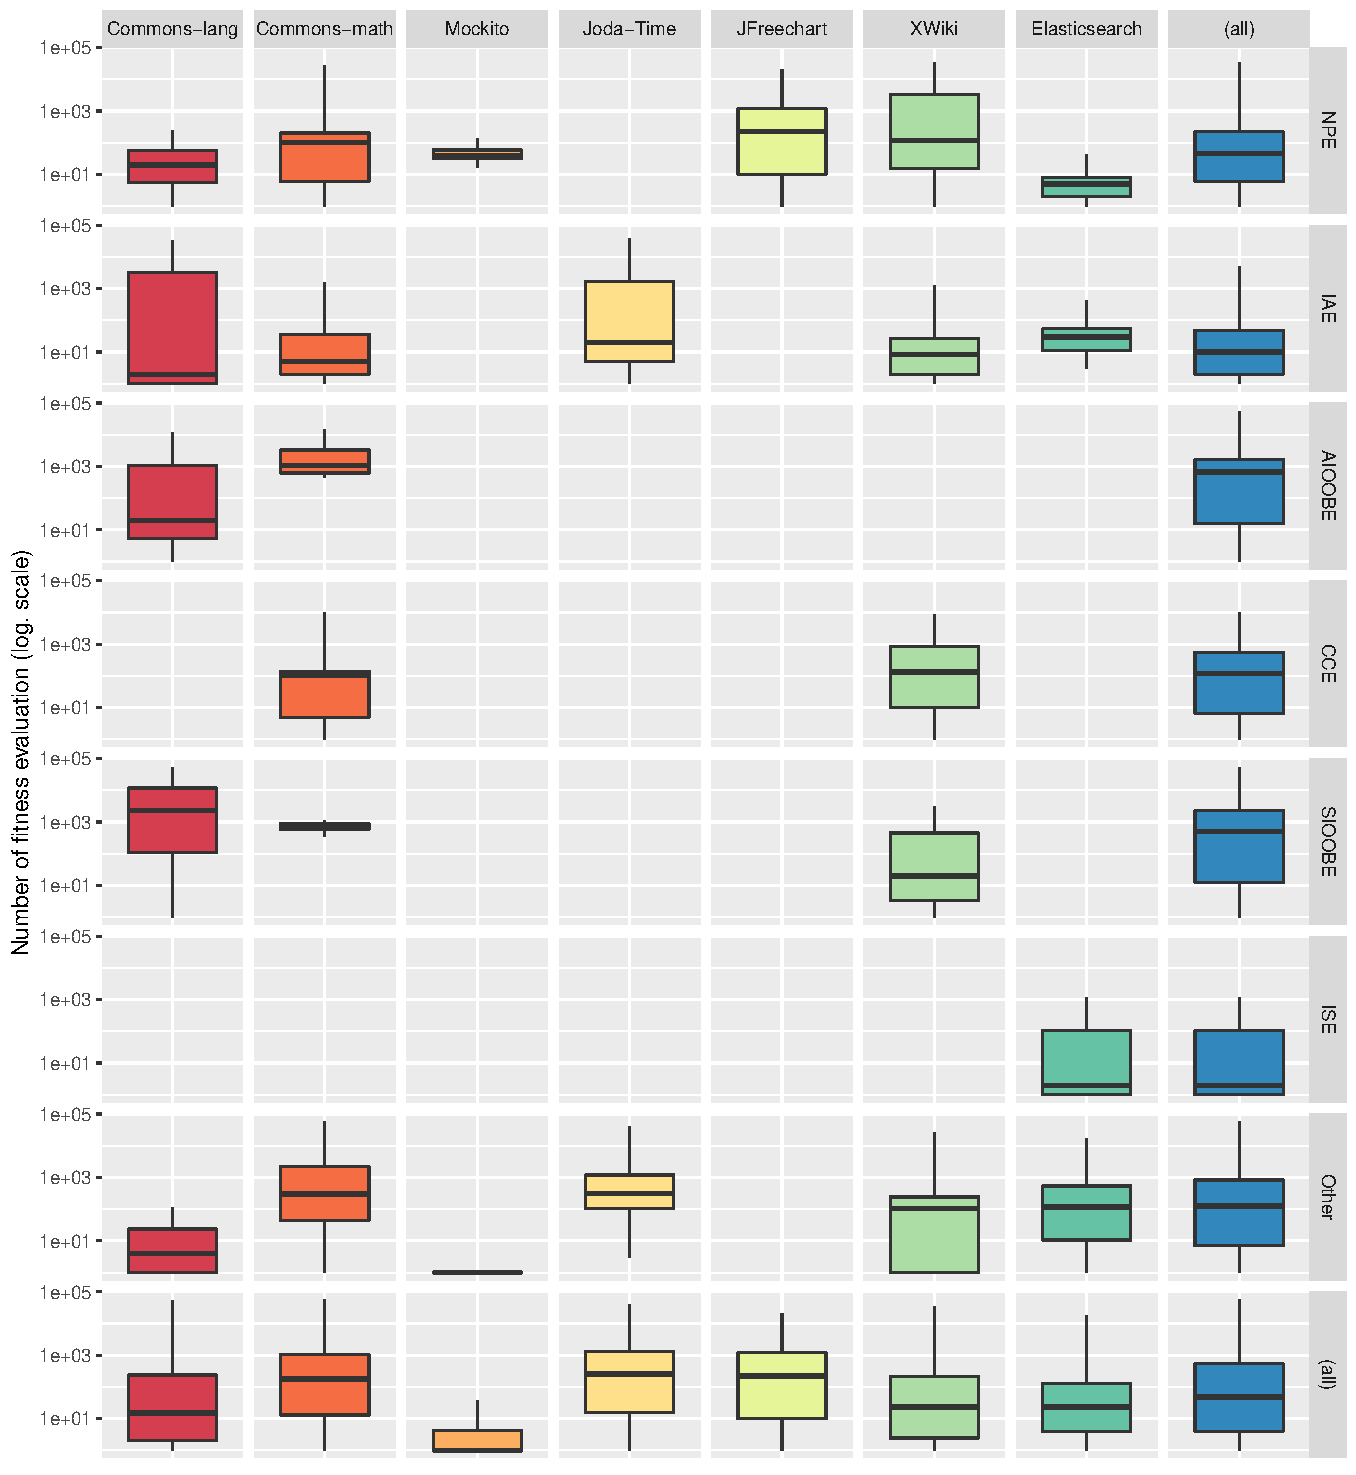
\includegraphics[width=\textwidth]{papers/jcrashpack/rq2_excepappstats.pdf}
	\caption{Average number of fitness evaluations for the \textit{reproduced} frames for each applications and exception type.}
	\label{figure:appexcepstats}
\end{figure*}

Considering the presented results in Figure~\ref{figure:outcomecomp} and Table~\ref{tab:appstats}, crash replication for various exceptions may be dependent on project type.
Figure~\ref{figure:appexcepstats} presents the results of crash reproduction grouped both by applications and exception types.
%
As the figure shows, the cost of reproducing NPE is lower for Elasticsearch, compared to XWiki and JFreechart, and the cost of reproducing IAE is lower for Commons-lang than for Elasticsearch.
We also observe differences in terms of costs of reproducing AIOOBE and SIOOBE for different projects.
%Our results suggest that further investigation in terms of possible correlations between application types and exception types are needed to be able to recommend a adequate number of fitness evaluations to \evocrash users when trying to reproduce a crash for a particular application.


\paragraph{\textbf{Summary (RQ$_{2.1}$)} How does project type influence performance of \evocrash for crash reproduction?}

%To summaries,  the median number of fitness evaluations required to reproduce a crash from Commons-lang, Mockito, XWiki, and Elasticsearch is low, compared to the median number of fitness evaluations needed to reproduce a crash from Commons-math, Joda-Time, and JFreechart. 

We observed that the factors are 
\begin{inparaenum}[(i)]
\item the complexity of the the project, and 
\item the level of the reproduced frames (reproducing higher frame requires more effort).
\end{inparaenum}
Furthermore, we see no link between the size of the project and the effort required to reproduce one of its crashes.


\paragraph{\textbf{Summary (RQ$_{2.2}$)} How does exception type influence performance of \evocrash for crash reproduction?}

For the exceptions, we observe that for ClassCastException, ArrayIndexOutOfBoundsException and StringIndexOutOfBoundsException, the cost of generating a crash-reproducing test case is high, while for NullPointerException, IllegalArgumentException, and IllegalStateException, the cost is lower.
This result indicates that the cost of reproducing types of exceptions for a non-trivial scenario (\textit{e.g.}, class conflicts or accessing an illegal state of an array) needs a more complex input generation. Furthermore, accessing the corresponding complex state is more time consuming for the search process.

